\documentclass[a4paper,10pt,openright,openbib,twocolumn]{article}
%\usepackage[portuges]{babel}
\usepackage[T1]{fontenc}
\usepackage{ae}
\usepackage[utf8]{inputenc}
\usepackage[pdftex]{graphicx}
\usepackage{url}
\usepackage{listings}
\usepackage{verbatim}
\usepackage{enumerate}
\usepackage[pdftex, bookmarks, colorlinks, linkcolor=black, urlcolor=blue]{hyperref} 
%\usepackage[a4paper,left=2.5cm,right=2.5cm,top=3.5cm,bottom=3.5cm]{geometry}
\usepackage[paper=a4paper,top=2cm,left=2cm,right=1.5cm,bottom=2cm,foot=1cm]{geometry}
\usepackage{colortbl}
\usepackage[margin=10pt,font=small,labelfont=bf]{caption}
\usepackage{mdwlist}
\usepackage{cleveref}
\usepackage{epsfig}

\usepackage{multicol}
\usepackage{appendix}
\usepackage{listings}



\setlength{\parindent}{0cm}
\setlength{\parskip}{2pt}


\begin{document}
\title{Study and Optimization of a Finite Volume Application}
\date{\today}
\begin{multicols}{2}
\author{
    Brito, Rui\\
    PG22781\\
    Department of Informatics\\
    University of Minho\\
    ruibrito666@gmail.com
  \and
    Alves, José\\
    PG22765\\
    Department of Informatics\\
    University of Minho\\
    zealves.080@gmail.com
}
\date{}
\maketitle
\end{multicols}

\begin{abstract}
    This report presents an analysis and details optimizations of a Diffusion-Convection application. This application uses a Finite Volume method to compute the heat diffusion in a fluid in an area of a surface. The optimizations made were: an optimized sequential version and a shared-memory OpenMP version.
    Speedups were only obtained on the sequential version. Although some structural optimizations were made in the sequential version, locality issues remained, turning the achieved results worse than the original version for the parallel version.
    Later in this report the results are compared joined with some speculation for on-going work.  
\end{abstract}

\section{Introduction}    %% Reler, corrigir algum erro

High-Performance Computing (HPC) has been a fundamental process to science, in order to make viable certain simulations that require massive amounts of calculation. The use of several optimization techniques has helped decrease the execution time of different algorithms, providing critical results faster, thus helping research move forward at a faster pace.

This report will describe a study of \emph{conv-diff} application with the objective of improving its performance. This application calculates the heat diffusion of a fluid while it spreads though an area through a Finite Volume method. 

This study approaches different ways to improve upon the initial solution. The project was devised in three stages. The first one was analyzing the original application, building its profile while also developing a better sequential version. The second stage was focused on a shared-memory parallel version, in (\emph{OpenMP}). Finally on the third stage, a naive CUDA version is being developed, taking advantage of the GPU's massive parallelism.

This report is organized in the following manner. \Cref{sec:casestudy} details the application's problem, explaining what aims to resolve and how it does it. \Cref{sec:profiling} shows the high workload areas which are addressed in the following sections for optimization. Next, in section \Cref{sec:test_methodology} we detail our test methology for this study.  \Cref{sec:sequentialopt} presents the first optimized version implemented followed by the second version made, this one parallel (using OpenMP) in section \Cref{sec:openmp}. In the end of this report, some considerations are made for the future work on \Cref{sec:futurework} and conclusion were taken in \Cref{sec:conclusion}

\section{Case Study}    %% Reler, corrigir algum erro, adicionar algo se te lembrares
\label{sec:casestudy}
The application analyzed for this study is \emph{conv-diff(Convection-Diffusion)}. This application simulates the way heat is transferred in a fluid using the finite-volumes method. To compute the heat diffusion, the surface is represented as a mesh. Being represented by cells and edges, the algorithm will traverse all edges, calculating the contribution of the adjacent cells. This application rests in a Finite Volume Library (FVLib), which handles the structures and some of the logic functions necessary for the problem's solution. 

The application's main objective is to compute a vector $\overline{\phi}$ such that $\overline{\phi} \longrightarrow G(\overline{\phi}) = \left(\begin{array}{c}
0\\ 
0\\
\vdots\end{array}\right)$
This is accomplished in three different stages:
\begin{enumerate}
    \item {We begin with a candidate vector $\phi$} 
    \item {For each edge, we compute the flux $F_{ij}$, with $i$ and $j$ being the indexes of the adjacent cells}
    \item {For each cell, we compute $\sum |e_{ij}| F_{ij} - |c_i| f_i$}
\end{enumerate}
Thus: $\phi = \left(\begin{array}{c}
\phi_1\\
\vdots\\
\phi_I
\end{array}\right) \longrightarrow G = \left(\begin{array}{c}
G_1\\
\vdots\\
G_I
\end{array}\right)$

\section{Profiling}    %% Reler, reestruturar e adicionar o que faltar
\label{sec:profiling}
The program consists in four major parts, reading the initial mesh from a file. Then, using the functions \emph{makeResidual}, which calls the function \emph{makeFlux}, the flux contributions are calculated and the vector phi is built, thus achieving a matrix free implementation. Following this, to calculate the deviation in the results from the previous operations, the function \emph{LUFactorize}. Finally, both the meshes are written to the output files, together with the error between them.
 
After analyzing the application, we conclude that the algorithm has a very high workload in the \emph{LUFactorize} function, comprising of more than 90\% of the execution time.
This is mostly because LUFactorize is a matrix implementation of the algorithm presented in the previous section. While it provides accurate results, it's memory usage, for example, make it unusable for big meshes. As an example, a mesh with more than fifty thousand cells will easily consume more than 10 GB of RAM. 


\section{Test Methodology} % (fold)
\label{sec:test_methodology}

In order to achieve precise and consistent results, all tests were run on a dedicated execution of the algorithm, with niceness set to -20, to ensure the tests execution was top priority to the OS's scheduler. Furthermore, all network connections were disabled. To decrease the chance of human error, all tests were hard-coded into a bash script, with another script traversing those tests and showing the results. Also, it should be noted that every test was run at least 3 times. A 5\% error margin was checked between execution (the aforementioned script handles this part), and if this margin is not met, the tests are run again. 

% section test_methodology (end)


\section{Sequential Optimization}
\label{sec:sequentialopt}

After dissecting the code and understanding the problem at hand, we began to notice several implementation errors, these errors, such as reading the same variable repeatedly from a file and long chains of calculation with a heavy division at the end, were easy to spot, and could clearly been avoided. We changed all those trivial aspects of the application, which required minimal effort. That being said, this simple optimizations paid results. The computation time has been greatly reduced, with the aforementioned \emph{LUFactorize} function taking an even more prominent role in our profile.

\begin{minipage}{.45\textwidth}
\lstset{
    language=C++,
    basicstyle=\ttfamily\small,
    breaklines=true
}
\begin{lstlisting}[caption=Excerpt from makeFlux]
    while((ptr_e=m.nextEdge())) {
        if(ptr_e->code == para.getUnsigned("DirichletCode")) {
            ...
        }
        if(ptr_e->code == para.getUnsigned("NeumannCode")) {
            ...
        }
    }
\end{lstlisting}
\end{minipage}

As can be seen from the code excerpt above, the code reads values from a structures called \emph{para} which holds all the parameter information read from the files. Moreover it can be seen that inside the while loop, two of those values are always being read. This was a trivial optimization

\begin{minipage}{.45\textwidth}
\lstset{
    language=C++,
    basicstyle=\ttfamily\small,
    breaklines=true
}
\begin{lstlisting}[caption=Another excerpt from makeFlux]    
    BB = ptr_e->centroid - ptr_e->leftCell->centroid;
    F[ptr_e->label-1] -= getDiffusion(ptr_e,para)*(rightPhi-leftPhi)/Norm(BB); 
\end{lstlisting}
\end{minipage}    

This is another alarming example. The last line of code presents a very heavy sequence of instructions. Actually, in our profile we measured that about 70\% of the time spent in that function amounts to that last line of code. What we did was remove the computation of BB to outside the loop, since it is a static variable, also, the computation done by \emph{getDiffusion} doesn't change in the loop, so we moved that outside as well. These changes changed the amount of time spent in that line to about 58\%. 
We tried to solve the division problem (since it can take many clock cycles) but to avail.

\begin{minipage}{.45\textwidth}
\lstset{
    language=C++,
    basicstyle=\ttfamily\small,
    breaklines=true
}
\begin{lstlisting}[caption=Fast Square-Root]    
    float InvSqrt(float x) {
        float xhalf = 0.5f * x;
        int i = *(int*)&x;
        i = 0x5f3759d5 - (i >> 1);
        x = *(float*)&i;
        x = x*(1.5f - xhalf*x*x);
        return x;
    }
\end{lstlisting}
\end{minipage} 

We found the above piece of code (an implementation of Newton's iterative method), when searching for ways to evade the division problem. The literature hinted at a 4 times speedup, but the results we got were worse than what we began with, so we ditched it.  
Also, just before starting the OpenMP version, we updated our gcc compiler so we could the latest version of the OpenMP library. Actually, the results we got improved dramatically when compiling with gcc 4.7.2. This is because newer versions of gcc are very good at vectorization and employ SLP (Sequential Linear Programming) techniques.

These are all the optimizations we attempted on the original sequential version. The original version, with a small input, took little over 14 seconds. With the optimizations mentioned and updated compiler, we brought it down to just 8 seconds. 

Below is table of results we got from PAPI, displaying the difference between the original version and the best sequential version. 
These results show the improvements our small changes to the source code got. By not computing the same value in every iteration of the loop and making those values constant, we gratly reduced the number of loads and stores and, consequently, the number of cache accesses. Althought we can't explain the decrease in the number of total instructions at this time. 

\begin{table}[!htp]
    \resizebox{\columnwidth}{!}{
        \begin{tabular}{|c|c|c|}
        \hline
            & original version & optimized sequential version\\
        \hline
            Total instructions & 2.517.584 & 285.551\\
            Load instructions & 630.156 & 86.532\\
            Store instructions & 326.459 & 39.208\\
            FP operations & 55.673 & 44.019\\
            L1 data accesses & 1.061.761 & 153.593\\
            L2 data accesses & 22.914 & 17.467\\
        \hline
        \end{tabular}}
    \caption{PAPI comparison}
    \label{tab:testcases}
\end{table}



\section{Shared Memory Parallel Optimization(OpenMP)}
\label{sec:openmp}
After optimizing the sequential code, we turned our efforts to parallelizing the code. The two loops responsible for the matrix free calculations were ideal candidates. We parallelized both these loops. We had some struggles with data-races in these, but we overcame the problems rather easily. The data-races exist because the mesh is traversed by the edges, however, as we found out, if they are traversed by cell, these data-races no longer exist. Also, the library that was provided includes some iterator style structures. These were also a problem, because, while OpenMP as no problem in parallelizing STL iterators, this doesn't hold true for \emph{FVlib}'s iterators. So, we had to convert those to a standard for loop, this way, the OpenMP library, knows which thread is to reveive the workload. The code was successfully parallelized, however, results were disappointing, execution time didn't decrease noticeably, hinting at a very memory bound application. 

\begin{minipage}{.45\textwidth}
\lstset{
    language=C++,
    basicstyle=\ttfamily\small,
    breaklines=true
}
\begin{lstlisting}[caption=Parallel part of makeFlux]    
    FVCell2D *ptr_c;     
    FVEdge2D *ptr_e;
    
    #pragma omp parallel for private(ptr_c,ptr_e)
    for(size_t i = 0; i < edges; i++) {        
        ptr_e = m.getEdge(i);
                
        ptr_c = ptr_e->leftCell;   
        #pragma omp atomic 
        G[ptr_c->label - 1] += F[ptr_e->label - 1];
        
        if((ptr_c = ptr_e->rightCell)) {
            #pragma omp atomic               
            G[ptr_c->label - 1] -= F[ptr_e->label - 1];    
        }        
    } 
\end{lstlisting}
\end{minipage} 

The above code shows the parallel code for the smallest function we could parallelize. As it can be seen from the example, there are two data-races in the parallel region. These data-races ensure that only one thread at a given time access the array G. As we said above, this problem isn't present in the traversal by cell. We implemented a traversal by cells, but it didn't improve much either which means that the problem is rooted at a lower level, the \emph{FVLib} itself. 

Below is a graph detailing the results we got for the parallel portion of the program. We ran this test on an Intel Xeon 5650, which has 12 physical cores and HyperThreading. As this processor has HT it got us wondering if it would scale any better in a processor with 24 physical cores, so we also ran the tests on an AMD Opteron 6174. Also, as most of the optimizations were made in a personal machine, we included those results as well. The faster times can be explained the the use of a recent compiler. The processor is an Intel Ivy Bridge i7 (2.3 GHz) with 4 physical cores. The slower times on the AMD machine can be explained by bad space locality. One of the strengths of the AMD processor is it's big cache, however, logically, if the program as bad locality, it will perform worse than in it's Intel counterpart. 
As it can be seen, the application doesn't scale at all as expected, this is because of the high number of memory accesses. Also, the deep indirection chain in \emph{FVLib} plays it's part. With every structure being a collection of pointers to other structures. These results hint at the kind of work we have to do next, improve data locality and remove unecessary pointers. This, of course, means re-implementing some of the structures in \emph{FVLib}.

\begin{figure}[!htp]
    \centering
    \begin{minipage}[t]{\columnwidth}
        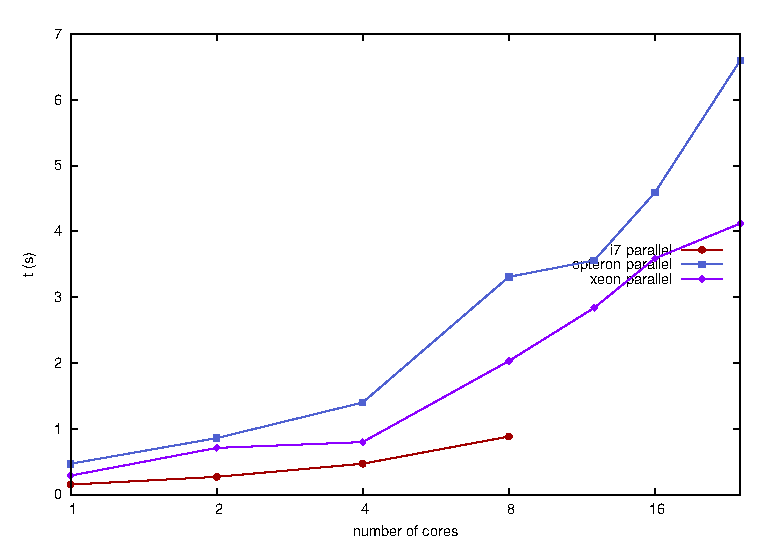
\includegraphics[width=\textwidth]{slides/images/parallel.eps}
        \caption{Scalability of the parallel region \label{fig:parallel}}
    \end{minipage}
\end{figure}

Below is a plot of the total execution times.


\begin{figure}[!htp]
    \centering
    \begin{minipage}[t]{\columnwidth}
        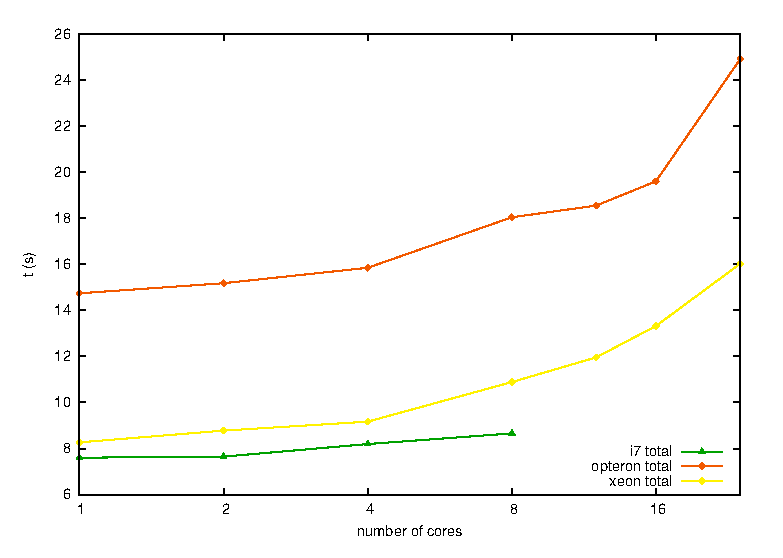
\includegraphics[width=\textwidth]{slides/images/total.eps}
        \caption{Total execution time \label{fig:total}}
    \end{minipage}
\end{figure}


\section{On-going and Future Work}    %% Reler, corrigir algum erro
\label{sec:futurework}
After implementing both the sequential version and the OpenMP version, a na\"{i}ve implementation in CUDA was started. This version aims to take advantage of the GPU's massive parallelism, improving performance using its vector units to diminish computation time. However, for this to be possible, a thorough restructuring of the code is necessary.This is because most of the structures are implemented using pointers, something that hinders CPU performance, but also makes it impossible to use CUDA, since we can't have a structure in the device memory pointing to host memory. Thus we are facing the challenge of removing most of the memory accesses while maintaining the abstraction and flexibility currently present in the application. After resolving this issue and other minor ones, we expect to achieve a boost in performance.

In future work, it is expected to develop an optimized CUDA version as well as an MPI version. A hybrid version using both CPU and GPU could also be a future implementation ideia, if it proves worthy performance wise. It is also expected to optimize several areas of code, questioning some decisions like using double-precision versus single-precision. Another area that might require attention is the input parser and the input file's structure. 

Moreover, we also want to focus some time in the calculation of the normal vector shown in \Cref{sec:sequentialopt}, as it is such a heavy part of the computation. Maybe an all assembly alternative is best chance we have of improving the square-root problem. Also, beucause \emph{LUFactorize} takes so much time, we plan in removing it from the source code, since it only there to check the result's correctness and the important part is the construction of the vector $G$ (\emph{makeResidual}), so, as we grow more confident in the results we get, the need to check their correctness is not present.

\section{Conclusion}
\label{sec:conclusion}
This report serves as an introduction to the study here presented. The results from the sequential optimized version shows some improvements in the total execution time.
However OpenMP results were disappointing, future iterations of the implementation may increase the improvements, shifting the application to a computing bound zone.

Through the development of the solutions some problems were presented, such as the mesh being disperse and the structures implemented with extensive use of pointers. This problems delayed the development of solutions, in particular the CUDA version. Maintaining the abstraction of the system may prove to be a bold decision, but favorable in terms of comprehension.
\end{document}
